\documentclass[a4paper, 11pt]{article}
\usepackage[utf8]{inputenc}
\usepackage[czech]{babel}
\usepackage[left=2.5cm, top=2cm, text={16cm, 25cm}]{geometry}
\usepackage{graphicx}
\usepackage{hyperref}

\begin{document}
\begin{center}
    {\Large
        Vysoké učení technické v~Brně \\
        Fakulta informačních technologií \\
    }
    
\includegraphics[width=0.4 \linewidth]{inc/FIT_logo.pdf} \\

    {\LARGE
        Mikroprocesorové a~vestavěné systémy \\
        Projekt\,--\,Hra na displeji \\[0.4cm]
    }

    {\large
        Martin Zmitko (xzmitk01) \\
        \texttt{xzmitk01@stud.fit.vutbr.cz} \\
        \today
    }
\end{center}
\vspace{0.7cm}

\section{Úvod}
Cílem tohoto projektu bylo vytvořit jednoduchou hru na displeji ovládanou analogovým joystickem.
Vybral jsem si Pong -- jednu z nejstarších her vůbec.
Tato hra funguje na principu tenisového zápasu, hrají proti sobě dva hráči, kteří ovládají vertikální pohyb pálek na stranách obrazovky a snaží se odpálit míček protihráčovi.

\subsection{Hardware}
Projekt byl řešen s pomocí předem zadaných hardwarových prvků:
\begin{itemize}
    \item Wemos D1 R32 -- vývojová deska s čipem ESP32\footnote{\url{https://www.espressif.com/sites/default/files/documentation/esp32_datasheet_en.pdf}}
    \item SSD1306\footnote{\url{https://cdn-shop.adafruit.com/datasheets/SSD1306.pdf}} -- jednobarevný OLED displej s rozlišením 128x64, komunikující přes rozhraní $I^2C$
    \item Analogový joystick -- joystick s dvěma osami pohybu, využívající ke čtení polohy potenciometrů
\end{itemize}
Displej je napájený 5V, k vývojové desce je zapojený přes rozhraní $I^2C$, připojený k pinům SDA a SCL (GPIO 22 a 21).
Joystick je napájen 3.3V (podle specifikace je stavěn na napájení 5V, ale ADC v ESP32 je schopný číst maximální napětí 3.3V, nebyl by tedy schopný přečíst celý rozsah joysticku) a k vývojové desce je připojený vývod osy X na pinu GPIO 36 (kanál 0 převodníku ADC1).

\subsection{Software}
K řešení projektu jsem použil rozhraní ESP-IDF\footnote{\url{https://docs.espressif.com/projects/esp-idf/en/latest/esp32/index.html}}.
Toto rozhraní poskytuje všechny potřebné nástroje a knihovny k překladu programů pro ESP32.
K interakci s periferiemi jsem použil vestavěné knihovny -- ADC one-shot driver pro čtení hodnot joysticku, I2C a LCD pro použití sběrnice a komunikaci s displejem.
Pro samotné zobrazování na displeji jsem použil externí knihovnu LVGL\footnote{\url{https://docs.lvgl.io/master/index.html}}.
LVGL je grafická knihovna pro vestavěné zařízení, umožňující snadné vykreslování, tvorbu uživatelských rozhraní s možnostmi stylování a zobrazování na základě stavů.

\section{Implementace}
Jako první po spuštění programu se provede konfigurace periferií.
Nastaví se rozhraní I2C pro správné piny s režimem master, poté se vytvoří nový handle pro LCD IO s parametry pro konkrétní displej -- zejména adresa displeje, velikosti ovládacích příkazů a frekvence.
Displej je poté inicializován a zapnut.

Další krok je inicializace LVGL -- nastavení barevné hloubky (v tomto případě je to 1b), nastavení parametrů displeje, vytvoření vlastních vykreslovacích bufferů (používají se dva, naráz jsou do jednoho ukládány nové data pro vykreslení a z druhého se čte, po dokončení se prohodí) a nastavení pomocných funkcí pro vykreslování.
Kód pro nastavení displeje a LVGL je převzatý z ESP-IDF ukázky\footnote{\url{https://github.com/espressif/esp-idf/tree/master/examples/peripherals/lcd/i2c_oled}}.

Pro čtení pozice joysticku je použit ADC modul v oneshot režimu, konkrétně jednotka ADC1 a kanál 0, který odpovídá GPIO 36. Je použitá výchozí bitová šířka a atenuace 11dB -- tedy rozsah čtení 0V-3.3V.

Samotný chod hry zajišťují 3 časovače periodicky spouštící obslužné funkce -- \texttt{lvgl\_tick} se spouští každé 2ms a dodává knihovně LVGL informace o uběhlém času pro vykreslování.
\texttt{draw\_tick} se spouští každých 10ms, obnoví pozice objektů na displeji na základě jejich nových souřadnic a změní text labelů se skórem, pokud se změnilo.

Herní logiku implementuje \texttt{game\_tick}, spouštěný každých 25ms.
Tato funkce nejdřív přečte napětí na joysticku jako raw hodnotu, kterou převede z původního intervalu $\langle0, 4095\rangle$ na interval $\langle-5, 5\rangle$, což je hodnota, o kterou se hráčova pálka vertikálně posune.
Pálka ovládaná počítačem se posune o 1, pokud je míček pod středem pálky, nebo o -1, pokud je míček nad středem pálky.
Pohyb míčku je zajišten proměnnými \texttt{ballDirectionX} a \texttt{ballDirectionY}, jejichž obsah se každý tick přičte k souřadnicím míčku.
\texttt{ballDirectionX} určuje horizontální pohyb a je vždy 2 nebo -2, \texttt{ballDirectionY} určuje vertikální pohyb, na začátku hry je 1 a při trefení pálky se počítá podle následujícího vztahu: $ballDirectionY = (ballY + 4 - paddleY) / 5 - 2$, pokud je výsledek 0, \texttt{ballDirectionY} se nezmění.
Pokud míček trefí jednu ze stran hracího prostoru, korespondující hodnotě direction je změněno znaménko.
Při strefení bočních stran hřiště proběhne kontrola, jestli míček zasáhl pálku, pokud ne, kolo se resetuje změněním polohy míčku do středu a přičtením jednoho bodu ke skóre druhého hráče.

\section{Zhodnocení}
Hra byla testována průběžným hraním a zkoušením, jak se bude chovat v různých situacích, např. při různých bodových stavech, různých polohách joysticku, nebo úhlech dopadu míčku na pálku.
Hra jako taková je plně funkční, nejsou v ní ale žádné koncové podmínky, bude tedy pokračovat do nekonečna.
Restartování hry taktéž není implementováno -- musí se restartovat celá vývojová deska.

Má autoevaluace je následující: \texttt{E=1, F=5, Q=3, P=1, D=3}

\begin{figure}[ht]
    \centering
    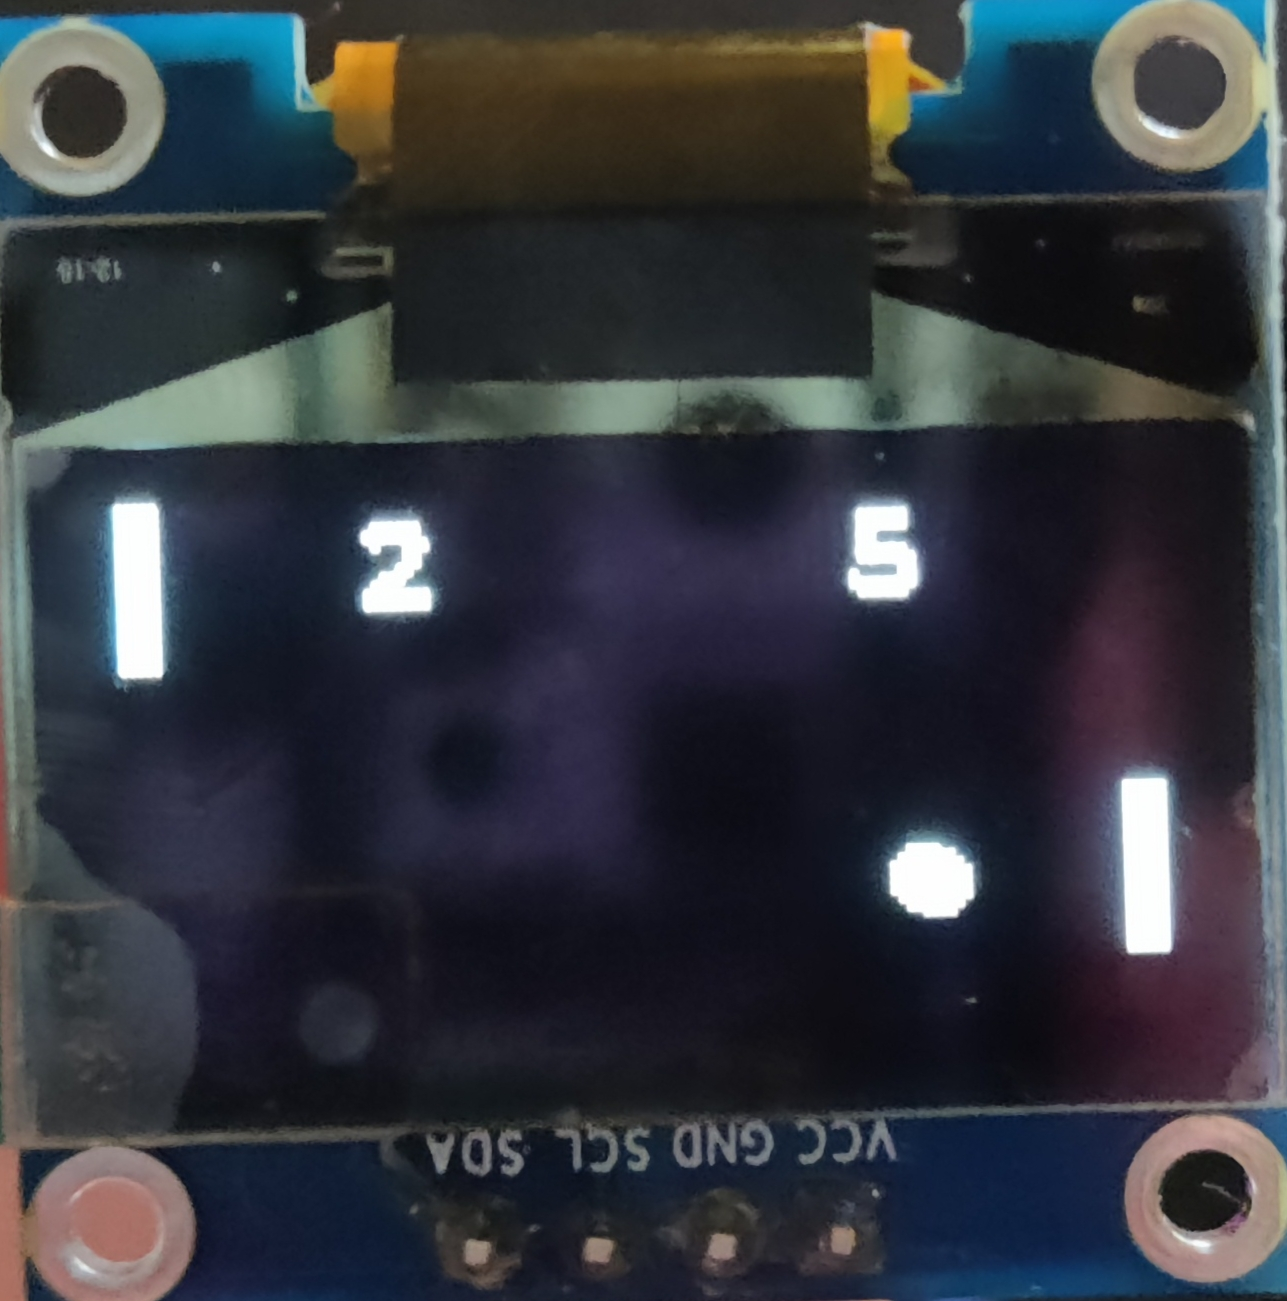
\includegraphics[width=0.7 \linewidth]{inc/img.jpg}
    \caption{Ukázka hotové hry}
\end{figure}
\end{document}
